\documentclass{article}
\usepackage[utf8]{vietnam}
\newif\ifanswers
\answerstrue % comment out to hide answers

\usepackage[compact]{titlesec}
\usepackage{fancyhdr} % Required for custom headers
\usepackage{lastpage} % Required to determine the last page for the footer
\usepackage{extramarks} % Required for headers and footers
\usepackage[usenames,dvipsnames]{color} % Required for custom colors
\usepackage{graphicx} % Required to insert images
\usepackage{listings} % Required for insertion of code
\usepackage{courier} % Required for the courier font
\usepackage{lipsum} % Used for inserting dummy 'Lorem ipsum' text into the template
\usepackage{enumerate}
\usepackage{enumitem}
\usepackage{subfigure}
\usepackage{booktabs}
\usepackage{amsmath, amsthm, amssymb}
\usepackage{caption}
\usepackage{hyperref}
\captionsetup[table]{skip=4pt}
\usepackage{framed}
\usepackage{bm}
\usepackage{minted}

\usepackage{tikz}
\usetikzlibrary{positioning,patterns,fit}
\usepackage{listings}
\usepackage{xcolor}

% Margins
\topmargin=-0.45in
\evensidemargin=0in
\oddsidemargin=0in
\textwidth=6.5in
\textheight=9.0in
\headsep=0.25in

\linespread{1.1} % Line spacing

% Set up the header and footer
\pagestyle{fancy}
\rhead{\hmwkAuthorName} % Top left header
\lhead{\hmwkClass: \hmwkTitle} % Top center head
\lfoot{\lastxmark} % Bottom left footer
\cfoot{} % Bottom center footer
\rfoot{Page\ \thepage\ of\ \protect\pageref{LastPage}} % Bottom right footer
\renewcommand\headrulewidth{0.4pt} % Size of the header rule
\renewcommand\footrulewidth{0.4pt} % Size of the footer rule

\setlength\parindent{0pt} % Removes all indentation from paragraphs

\newenvironment{answer}{
    % Uncomment this if using the template to write out your solutions.
    {\bf Answer:} \sf \begingroup\color{black}
}{\endgroup}% 
%----------------------------------------------------------------------------------------
%	CODE INCLUSION CONFIGURATION
%----------------------------------------------------------------------------------------

\definecolor{MyDarkGreen}{rgb}{0.0,0.4,0.0} % This is the color used for comments
\definecolor{shadecolor}{gray}{0.9}

% \lstloadlanguages{Python} % Load Perl syntax for listings, for a list of other languages supported see: ftp://ftp.tex.ac.uk/tex-archive/macros/latex/contrib/listings/listings.pdf
\lstset{language=C++,
        frame=single,
        basicstyle=\ttfamily,
        keywordstyle=\color{blue}\ttfamily,
        stringstyle=\color{red}\ttfamily,
        commentstyle=\usefont{T1}{pcr}{m}{sl}\color{MyDarkGreen},
        morecomment=[l][\color{magenta}]{\#}
        tabsize=4, 
}
% \lstset{language=C++, % Use Perl in this example
%         frame=single, % Single frame around code
%         basicstyle=\footnotesize\ttfamily, % Use small true type font
%         keywordstyle=[1]\color{Blue}\bf, % Perl functions bold and blue
%         keywordstyle=[2]\color{Purple}, % Perl function arguments purple
%         keywordstyle=[3]\color{Blue}\underbar, % Custom functions underlined and blue
%         identifierstyle=, % Nothing special about identifiers
%         commentstyle=\usefont{T1}{pcr}{m}{sl}\color{MyDarkGreen}\small, % Comments small dark green courier font
%         stringstyle=\color{Purple}, % Strings are purple
%         showstringspaces=false, % Don't put marks in string spaces
%         tabsize=5, % 5 spaces per tab
%         %
%         % Put standard Perl functions not included in the default language here
%         morekeywords={rand},
%         %
%         % Put Perl function parameters here
%         morekeywords=[2]{on, off, interp},
%         %
%         % Put user defined functions here
%         morekeywords=[3]{test},
%        	%
%         morecomment=[l][\color{Blue}]{...}, % Line continuation (...) like blue comment
%         numbers=left, % Line numbers on left
%         firstnumber=1, % Line numbers start with line 1
%         numberstyle=\tiny\color{Blue}, % Line numbers are blue and small
%         stepnumber=5 % Line numbers go in steps of 5
% }
% Creates a new command to include a perl script, the first parameter is the filename of the script (without .pl), the second parameter is the caption
\newcommand{\perlscript}[2]{
\begin{itemize}
\item[]\lstinputlisting[caption=#2,label=#1]{#1.pl}
\end{itemize}
}

%----------------------------------------------------------------------------------------
%	NAME AND CLASS SECTION
%----------------------------------------------------------------------------------------

\newcommand{\hmwkTitle}{Tiến trình (Processes)} % Assignment title
\newcommand{\hmwkClass}{INT2214 Bài tập \#2} % Course/class
\newcommand{\hmwkAuthorName}{Nguyễn Thành Đô - 19020250} % Your name

\newcommand{\ifans}[1]{\ifanswers \color{red} \vspace{5mm} \textbf{Solution: } #1 \color{black} \vspace{5mm} \fi}

% Chris' notes
\definecolor{CMpurple}{rgb}{0.6,0.18,0.64}
\newcommand\cm[1]{\textcolor{CMpurple}{\small\textsf{\bfseries CM\@: #1}}}
\newcommand\cmm[1]{\marginpar{\small\raggedright\textcolor{CMpurple}{\textsf{\bfseries CM\@: #1}}}}
\titlespacing{\section}{-25pt}{*4}{*1.5}

%----------------------------------------------------------------------------------------
%	TITLE PAGE
%----------------------------------------------------------------------------------------
\title{
\vspace{-1in}
\textmd{\textbf{\hmwkClass:\ \hmwkTitle} \\ \hmwkAuthorName}\\ 
}
\author{\textbf{Giảng viên: } Bùi Duy Hiếu}
%\date{\textit{\small Updated \today\ at \currenttime}} % Insert date here if you want it to appear below your name
\date{}

\setcounter{section}{0} % one-indexing
\begin{document}

\maketitle
\vspace{-.4in}

\begin{center}
    \large{\textbf{Hạn nộp:} Thứ hai, 07/03/2022 trước \textbf{23h:59'}}
\end{center}

\section{Bài toán Nhà sản xuất – Người dùng}
\textit{Hai tiến trình chia sẻ một vùng đệm có kích thước cố định, trao đổi với nhau qua phương thức trao đổi
    thông điệp. Nhà sản xuất muốn đưa thông tin lên vùng đệm, còn người dùng muốn lấy thông tin từ vùng đệm.
    Giả định tình huống vùng đệm đầy mà nhà sản xuất vẫn muốn đưa thông tin lên. Vậy nhà sản xuất phải
    chuyển sang trạng thái ngủ, được đánh thức bởi người dùng khi họ lấy thông tin từ vùng đệm. Tương tự, khi vùng đệm
    trống và người dùng muốn lấy thông tin từ vùng đệm, thì người dùng sẽ chuyển sang trạng thái ngủ và được đánh thức
    bởi nhà sản xuất khi họ đưa thông tin lên vùng đệm.} \\

\textbf{Yêu cầu: }Viết chương trình minh hoạ cho tình huống trên.
\subsection{Giới thiệu vấn đề}
Truyền thông liên tiến trình sử dụng bộ nhớ dùng chung (interprocess communication)
yêu cầu các tiến trình phải thiết lập một vùng bộ nhớ dùng chung. Thông thường, bộ
nhớ chung nằm ở không gian địa chỉ của tiến trình khởi tạo ra bộ nhớ đó. Các tiến
trình khác muốn truyền thông sử dụng bộ nhớ chung này phải liên kết nó vào không
gian địa chỉ của các tiến trình này. Bình thường hệ điều hành sẽ cố gắng ngăn chặn
một tiến trình truy cập vào bộ nhớ của một tiến trình khác, do đó bộ nhớ chung yêu
cầu các tiến trình phải tháo bỏ ràng buộc này. Sau đó chúng có thể trao đổi thông
tin bằng cách đọc và ghi dữ liệu lên bộ nhớ chung. \\

Bài toán Nhà sản xuất - Người dùng minh họa cho khái niệm truyền thông liên tiến trình,
ở đó nhà sản xuất và người dùng phải được \textbf{đồng bộ hóa}, để tránh trường hợp
người dùng cố gắng lấy thông tin mà chưa được đưa lên vùng đệm. Tuy nhiên, cách tiếp cận bài toán này
sẽ tạm thời bỏ qua vấn đề liên quan đến tình huống trong đó cả nhà sản xuất và người dùng
đều cố gắng truy cập đồng thời bộ đệm dùng chung.
\subsection{Thiết kế và cài đặt}
Code đầy đủ được cung cấp tại: \href{www.github.com}{github.com}
\subsubsection{Hướng tiếp cận 1}

Bộ đệm chung được cài đặt như một array xoay vòng với hai con trỏ \textit{in} và
\textit{out}. Biến \textit{in} trỏ tới vị trí còn trống tiếp theo trong bộ đệm;
biến \textit{out} trỏ tới vị trí đầy (có chứa item được đưa lên bởi nhà sản xuất)
đầu tiên trong bộ đệm. Nhà sản xuất và người dùng được cài đặt như hai luồng chạy
song song, nhận biết trạng thái của bộ đệm thông qua hai biến \textit{in} và \textit{out}
để thực hiện các hành vi phù hợp. Cụ thể, bộ đệm sẽ được hiểu là rỗng khi \textit{in}
== \textit{out}; và bộ nhớ được hiểu là đầy khi ((\textit{in} + 1) \% BUFFER\_SIZE)
== \textit{out}. \\

Để mô phỏng nhà sản xuất và người dùng, cài đặt hai threads chạy song song với
dữ liệu toàn cục \textit{buffer} được sử dụng, cụ thể trong Hình 1 và Hình 2.
Thread "nhà sản xuất" có một biến cục bộ \textit{produced} chứa item mới chuẩn bị
được đưa lên bộ đệm; thread "người dùng" có một biến cục bộ \textit{consumed} chứa
item chuẩn bị được người dùng lấy về.

\pagebreak

\begin{shaded}
    \begin{lstlisting}
void *producer(void *args){
    while (1){
        int produced = rand() % 100;
        while ((in + 1) % BUFFER_SIZE == out){
            // buffer is full, do nothing
            printf("Buffer is full: %d/%d slots are occupied\n",
                   in - out >= 0 ? (in - out) : BUFFER_SIZE - (out - in), 
                   BUFFER_SIZE);
            sleep(1);
        }
        buffer[in] = produced;
        in = (in + 1) % BUFFER_SIZE; 
        printf("produced: %d, %d/%d slots are occupied\n", produced, 
        in - out >= 0 ? (in - out) : BUFFER_SIZE - (out - in), BUFFER_SIZE);
        sleep(1);
    }
    return 0;
}
    \end{lstlisting}
\end{shaded}

\begin{figure}[h]
    \centering
    \caption{Code cho nhà sản xuất \#1}
\end{figure}

\begin{shaded}
    \begin{lstlisting}
void *consumer(void *args){
    while (1){
        while (in == out){
            // buffer is empty, do nothing
            printf("Buffer is empty: %d/%d slots are occupied\n",
                    in - out >= 0 ? (in - out) : BUFFER_SIZE - (out - in), 
                        BUFFER_SIZE);
            sleep(1);
        }
        int consumed = buffer[out];
        out = (out + 1) % BUFFER_SIZE;
        printf("consumed: %d, %d/%d slots are occupied\n", consumed, 
        in - out >= 0 ? (in - out) : BUFFER_SIZE - (out - in), BUFFER_SIZE);
        sleep(2);
    }
    return 0;
}
    \end{lstlisting}
\end{shaded}

\begin{figure}[h]
    \centering
    \caption{Code cho người dùng \#1}
\end{figure}

\pagebreak

Thử chạy chương trình với 2 testcases (Hình 3), tương ứng với hai trường hợp tốc độ đưa item
lên lớn hơn tốc độ lấy item về (testcase 1), và ngược lại (testcase 2). Dễ nhận thấy, cách cài đặt này chỉ cho phép
tối đa BUFFER\_SIZE - 1 items cùng tồn tại ở trên bộ đệm. Điều này thể hiện rõ qua kết quả chạy thử
testcase 1, với BUFFER\_SIZE = 5 thì chỉ có tối đa 4/5 bộ đệm được chiếm giữ. Mặt khác vấn đề
đồng bộ hóa cũng chưa được giải quyết bằng cách cài đặt này, như có thể thấy trong hai dòng đầu tiên
của testcase 1: chương trình in ra sự kiện "consumed: 97" trước sự kiện "produced: 97".
\begin{figure}[h]
    \centering

    \subfigure[Testcase 1: $ v_{produce} > v_{consume} $]{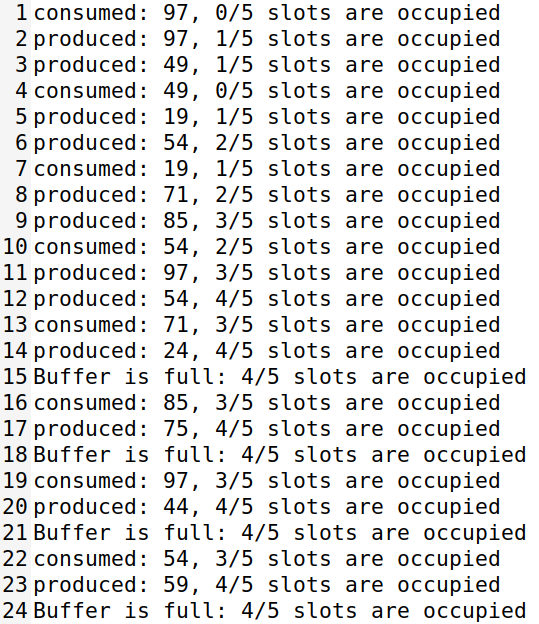
\includegraphics[width=0.45\textwidth]{bb_testcase_1.png}}
    \subfigure[Testcase 2: $ v_{produce} < v_{consume} $]{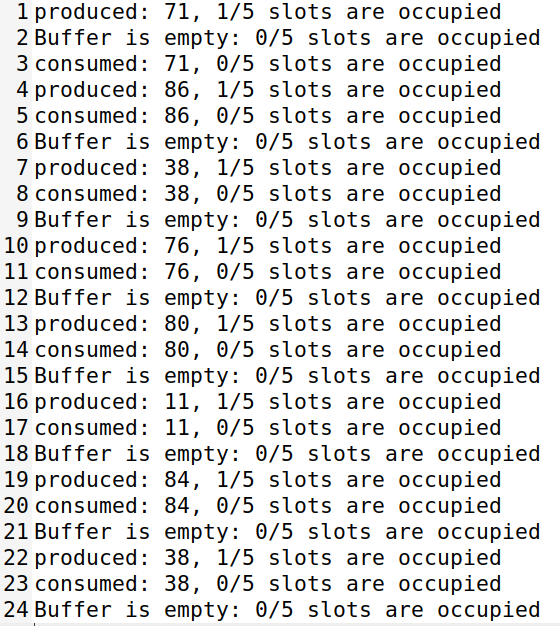
\includegraphics[width=0.462\textwidth]{bb_testcase_2.png}}
    \caption{Kết quả thử nghiệm \#1}
\end{figure}

\subsubsection{Hướng tiếp cận 2}
Hướng tiếp cận này sẽ cải thiện việc sử dụng không gian bộ nhớ chưa hiệu quả
của hướng tiếp cận trước. Với mục đích đó, ta có thể thêm một biến đếm \textit{count},
được khởi tạo với giá trị 0. \textit{count} được tăng lên mỗi khi nhà sản xuất thêm
dữ liệu vào bộ đệm và được giảm xuống mỗi khi người dùng lấy dữ liệu ra khỏi bộ đệm.
Code cho nhà sản xuất và người dùng được điều chỉnh như sau dưới đây (Hình 4-5). \\

Với sự điều chỉnh này, nhà sản xuất và người dùng có thể  đặt được hiệu quả tối ưu (sử dụng được tối đa BUFFER\_SIZE kích thước bộ đệm)
nếu hoạt động tách biệt nhau. Nhưng ngược lại, chúng có thể  gây ra lỗi nếu như hoạt động
đồng thời. Ví dụ, giả sử giá trị của biến \textit{count} = 5, khi đó nhà sản xuất
và người dùng đồng thời thực các đoạn lệnh \textit{count++} và \textit{count\---\---}.
Tùy theo thứ tự thực hiện các đoạn lệnh này ở mức độ ngôn ngữ máy, mà giá trị của
\textit{count} có thể nhận được là 4, 5 hoặc 6. Tuy nhiên khi chạy thử cài đặt này, trong
giới hạn thời gian chạy 10000000 vòng lặp, chúng ta vẫn chưa gặp phải vấn đề này.

\pagebreak

\begin{shaded}
    \begin{lstlisting}
void *producer(void *args){
    while (1){
        int produced = rand() % 100;
        while (count == BUFFER_SIZE){
            printf("Buffer is full, count = %d\n", count);
            sleep(1);
        }

        buffer[in] = produced;
        in = (in + 1) % BUFFER_SIZE;
        count++;
        printf("produced: %d, count = %d\n", produced, count);
        sleep(1);
    }
    return 0;
}
    \end{lstlisting}
\end{shaded}

\begin{figure}[h]
    \centering
    \caption{Code cho nhà sản xuất \#2}
\end{figure}

\begin{shaded}
    \begin{lstlisting}
void *consumer(void *args){
    while (1){
        while (count == 0){
            printf("Buffer is empty, count = %d\n", count);
            sleep(2);
        }
        // do nothing
        int consumed = buffer[out];
        out = (out + 1) % BUFFER_SIZE;
        count--;
        printf("consumed: %d, count = %d\n", consumed, count);
        sleep(2);
    }

    return 0;
}
    \end{lstlisting}
\end{shaded}

\begin{figure}[h]
    \centering
    \caption{Code cho người dùng \#2}
\end{figure}

\begin{figure}[h]
    \centering

    \subfigure[Testcase 3: $ v_{produce} > v_{consume} $]{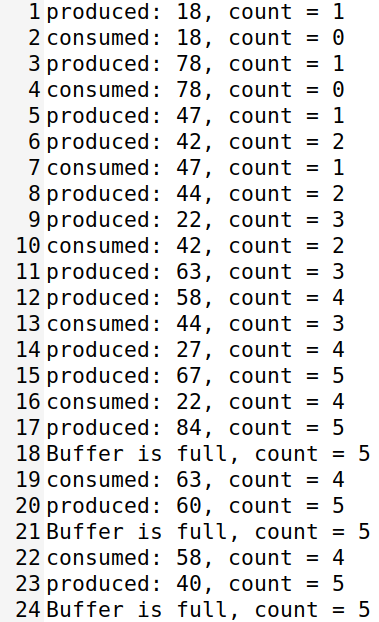
\includegraphics[width=0.35\textwidth]{bb_testcase_3.png}}
    \subfigure[Testcase 4: $ v_{produce} < v_{consume} $]{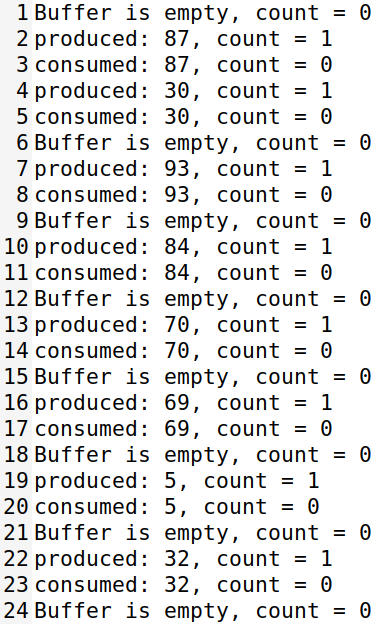
\includegraphics[width=0.35\textwidth]{bb_testcase_4.png}}
    \caption{Kết quả thử nghiệm \#2}
\end{figure}

\section{Bài toán Bữa ăn của các nhà triết học}
\textit{Có 5 nhà triết học ngồi trong một chiếc bàn tròn. Mỗi nhà triết học có một đĩa spaghetti. Vì spaghetti
    rất trơn nên mỗi nhà triết học phải dùng 2 chiếc nĩa để ăn. Giữa hai đĩa spaghetti chỉ có một chiếc nĩa.
    Vòng đời của nhà triết học là một chuỗi liên tiếp ăn và nghĩ. Khi nhà triết học đói, họ sẽ lấy nĩa bên trái
    và phải của minh cùng lúc. Nếu thành công, họ sẽ ăn một lúc rồi để nĩa xuống, rồi tiếp tục nghĩ.} \\

\textbf{Yêu cầu: }Viết chương trình mô phỏng hành động các nhà triết học trên sao cho không xảy ra tình huống bế tắc.
\subsection{Giới thiệu vấn đề}
Bài toán Bữa ăn của các nhà triết học (the dining philosophers problem) là một bài toán kinh điển về đồng bộ hóa.
Bản thân bài toán không mang ý nghĩa thực tế quan trọng gì hay thể hiện sự mỉa mai của các nhà khoa học máy tính lên các nhà triết học,
mà nó chỉ là một minh họa đơn giản cho nhu cầu cấp phát các tài nguyên cho các tiến trình khác nhau, sao cho không xảy ra
hiện tượng \textbf{deadlock} và \textbf{starvation}. \\

Có một điều quan trọng trong ngữ cảnh bài toán này đó là, nhà triết học không thể một lúc nhấc hai chếc nĩa được mà phải làm lần lượt:
nhấc nĩa trái trước rồi đến nĩa phải, hoặc ngược lại. Hiện tượng deadlock xảy ra khi, tất cả các nhà triết học cùng một lúc nhấc một chiếc nĩa,
và tiếp theo không thể nhấc thêm cái thứ hai và phải chờ mãi mãi, do đó tất cả các nhà triết học sẽ chết đói (starvation). Để mô phỏng
lại bài toán, chúng ta sẽ giả sử  hành động của các nhà triết học là đồng bộ (tức là một lúc hai nhà triết học sẽ không cùng lấy một cái nĩa,
gây ra xung đột) và tập trung vào giao thức giao tiếp giữa họ. \\


\begin{shaded}

    \begin{lstlisting}
        while (true) {
            /* think for a while */
            think();
            /* calls pickup to pick up the forks */
            pickup(); // pick up the forks
            /* eat for a while */
            eat();
            /* the philosopher is done eating, 
                and calls putdown to put down the forks */
            putdown();

        }
    \end{lstlisting}
\end{shaded}

\begin{figure}[h]
    \centering
    \caption{Minh họa cách hoạt động của nhà triết học}
\end{figure}

\subsection{Thiết kế và cài đặt}
Code đầy đủ được cung cấp tại: \href{www.github.com}{github.com} \\

Phần cài đặt này tham khảo chủ yếu từ \href{https://web.archive.org/web/20120722014159/http://web.eecs.utk.edu/~plank/plank/classes/cs560/560/notes/Dphil/lecture.html}{C560 Lecture notes -- Dining Philosophers},
có sử dụng các kỹ thuật \textbf{mutex, semaphore, monitor} để đảm bảo sự đồng bộ giữa các nhà triết học. Tuy nhiên báo cáo này sẽ chỉ tận dụng
các kỹ thuật trên mà không giải thích, nguyên nhân là do giới hạn kiến thức của người viết trong thời gian thực hiện báo cáo. Thay vào đó, báo cáo
sẽ tập trung vào thiết kế logic cách nhà triết học hoạt động, cụ thể là cách cài đặt các hàm \textit{think()}, \textit{pickup()},
\textit{eat()} và \textit{putdown()}. \\

Mặt khác, không ai có thể quyết định một nhà triết học sẽ ăn và nghĩ lúc nào, trong bao lâu
(thực ra vẫn cần giới hạn thời gian ăn tối đa của nhà triết học, giống như việc không thể để một process chiếm tài nguyên CPU mãi được.) Hàm
\textit{think()} và \textit{eat()} được cài đặt dựa trên ý tưởng nhà triết học sẽ ăn và nghĩ trong một khoảng thời gian ngẫu nhiên, trong một giới hạn
MAX\_TIME cho trước. Các lời giải khác nhau sẽ chỉ khác nhau ở cách cài đặt hai hàm \textit{pickup()} và \textit{putdown()}.
\begin{shaded}
    \begin{lstlisting}
        void think() {
            duration = (random() % MAX_TIME) + 1;
            sleep(duration);
        }
        void eat() {
            duration = (random() % MAX_TIME) + 1;
            sleep(duration);
        }
    \end{lstlisting}
\end{shaded}

\begin{figure}[h]
    \centering
    \caption{Cài đặt hàm \textit{think()} và \textit{eat()}}
\end{figure}

Đồng thời để đánh giá hiệu quả từng cài đặt, thông tin về thời gian chờ của từng nhà triết học (tổng thời gian những khoảng chờ từ lúc muốn ăn cho đến
lúc có đủ nĩa để ăn) sẽ được ghi lại.
\subsubsection{Hướng tiếp cận đơn giản và hiện tượng deadlock}
Trong hướng tiếp cận này, đơn giản mỗi nhà triết học sẽ thực hiện việc ăn theo quy trình sau: đầu tiên kiểm tra xem nĩa bên trái có ai dùng không, nếu có thì đợi,
nếu không thì cầm nĩa lên, sau đó làm tương tự với nĩa bên phải; sau khi ăn xong thì đặt nĩa phải xuống trước, rồi sau đó đến nĩa trái (Hình 9).
Cách tiếp cận này không ngăn chặn được hiện tượng deadlock, tuy nhiên khi chạy thử sẽ không gặp phải tình huống đó bởi vì sự ngẫu nhiên trong
thời gian ăn và nghĩ của của từng nhà triết học. Deadlock chỉ xảy ra khi tất cả nhà triết học bị chen ngang (preempted) giữa lúc nhấc hai chiếc nĩa,
dẫn đến mỗi người bọn họ chỉ cầm được một chiếc nĩa và sẽ chờ để có chiếc nĩa thứ hai cho đến khi chết đói. Do vậy để mô phỏng tình huống này ta chỉ
cần thêm một khoảng chờ đủ lâu giữa hai lần nhấc nĩa (Hình x).

\begin{shaded}
    \begin{lstlisting}
typedef struct forks {
    pthread_mutex_t **lock; // for synchronization
    int phil_count; // number of philosophers, = 5 in this case
} Forks;
// a Phil_struct struct contains information of a philosopher
void pickup(Phil_struct *ps) { 
    Forks *forks;
    int phil_count;

    forks = (Forks *)ps->v; // get info of forks of the philosphers
    phil_count = forks->phil_count;   
    /* pick up left fork and make sure others won't try to pick it, 
     in other words, lock up left fork */
    pthread_mutex_lock(forks->lock[ps->id]); 
    /* pick up and lock up right fork */
    pthread_mutex_lock(forks->lock[(ps->id + 1) % phil_count]); 
}

void putdown(Phil_struct *ps) {
    Forks *forks;
    int i;
    int phil_count;

    forks = (Forks *)ps->v;
    phil_count = forks->phil_count;    
    /* release the right fork after done eating, 
        in other words, unlock right fork */
    pthread_mutex_unlock(forks->lock[(ps->id + 1) % phil_count]); 
    /* unlock left fork */
    pthread_mutex_unlock(forks->lock[ps->id]);                    
}
    \end{lstlisting}
\end{shaded}

\begin{figure}[h]
    \centering
    \caption{Cài đặt đơn giản hàm \textit{pickup()} và \textit{putdown()}}
\end{figure}

Kết quả chạy thử với 5 nhà triết học, thời gian ăn/nghĩ tối đa 10 giây, trong tổng cộng 2100 giây
không cho thấy deadlock. Kết quả đầy đủ của lần chạy mẫu này được cung cấp trong file \href{www.github.com}{dp2.txt},
với tổng thời gian chờ được ghi lại tại dòng cuối như sau:
\begin{minted}{text}
            2100 Total blocktime:  5165 :  1026  1041  1047  1042  1009
\end{minted}

Tuy nhiên, như đã nói, để mô phỏng tình huống deadlock chúng ta có thể để thời gian giữa hai lần nhấc nĩa là 5 giây.
Cụ thể ta có thể điều chỉnh một phần code của hàm \textit{pickup()} như sau:
\begin{shaded}
    \begin{lstlisting}
    pthread_mutex_lock(forks->lock[ps->id]); 
    sleep(5);
    pthread_mutex_lock(forks->lock[(ps->id + 1) % phil_count]); 
    \end{lstlisting}
\end{shaded}
\begin{figure}[h]
    \centering
    \caption{Cài đặt hàm \textit{pickup()} mô phỏng tình huống deadlock}
\end{figure}
Khi chạy thử ta có thể thấy hiện tượng deadlock xảy ra ngay trong 10 giây đầu tiên:
\begin{minted}{text}
        0 Philosopher 0 thinking for 4 seconds
        0 Philosopher 1 thinking for 3 seconds
        0 Philosopher 2 thinking for 5 seconds
        0 Philosopher 3 thinking for 6 seconds
        0 Philosopher 4 thinking for 2 seconds
        0 Total blocktime:     0 :     0     0     0     0     0 
        2 Philosopher 4 no longer thinking -- calling pickup()
        3 Philosopher 1 no longer thinking -- calling pickup()
        4 Philosopher 0 no longer thinking -- calling pickup()
        5 Philosopher 2 no longer thinking -- calling pickup()
        6 Philosopher 3 no longer thinking -- calling pickup()
        10 Total blocktime:    30 :     6     7     5     4     8 
        20 Total blocktime:    80 :    16    17    15    14    18 
        30 Total blocktime:   130 :    26    27    25    24    28 
\end{minted}

\begin{figure}[h]
    \centering
    \caption{Kết quả chạy thử mô phỏng tình huống deadlock}
\end{figure}
\subsubsection{Lời giải không đối xứng}
Để giải quyết vấn đề deadlock chỉ cần điều chỉnh nhỏ so với cách cài đặt trước: chỉ các nhà triết học được đánh số lẻ
bắt đầu nhấc nĩa trái trước, trong khi đó các nhà triết học được đánh số chẵn sẽ bắt đầu với nĩa phải trước; tương tự
ai số lẻ sẽ đặt nĩa phải xuống trước, ai số chẵn sẽ đặt nĩa trái xuống trước (Hình 12). Sự không đồng đều này
giải thích cho cái tên "lời giải không đối xứng."
Với thuật toán này, deadlock sẽ không xảy ra kể cả khi ta có thêm một khoảng delay giữa hai lần nhấc nĩa.
Lí giải cho sự hiệu quả của thuật toán này khá đơn giản, với quy luật được mô tả như trên thì nếu tất cả
các nhà triết học cùng muốn ăn một lúc, thì sẽ luôn có người phải chờ người khác ăn xong rồi mới có thể nhấc
chiếc dĩa đầu tiên lên được, cho nên không thể xảy ra trường hợp mỗi nhà triết học đều cầm một chiếc nĩa một lúc.
\begin{shaded}
    \begin{lstlisting}
void pickup(Phil_struct *ps) {
  Forks *pp;
  int phil_count;
  pp = (Forks *) ps->v;
  phil_count = pp->phil_count;
  
  if (ps->id % 2 == 1) { // odd labeled philosopher
    /* lock up left fork */
    pthread_mutex_lock(pp->lock[ps->id]);
    /* lock right fork */       
    pthread_mutex_lock(pp->lock[(ps->id+1)%phil_count]); 
  } else { // even labeled philosopher
    /* lock right fork */ 
    pthread_mutex_lock(pp->lock[(ps->id+1)%phil_count]); 
    /* lock up left fork */
    pthread_mutex_lock(pp->lock[ps->id]);       
  }
}

void putdown(Phil_struct *ps) {
  Forks *pp;
  int i;
  int phil_count;
  pp = (Forks *) ps->v;
  phil_count = pp->phil_count;

  if (ps->id % 2 == 1) { // odd labeled philosopher
    /* unlock right fork */ 
    pthread_mutex_unlock(pp->lock[(ps->id+1)%phil_count]); 
    /* unlock left fork */
    pthread_mutex_unlock(pp->lock[ps->id]); 
  } else { // even labeled philosopher
    /* unlock left fork */
    pthread_mutex_unlock(pp->lock[ps->id]);  
    /* unlock right fork */ 
    pthread_mutex_unlock(pp->lock[(ps->id+1)%phil_count]);
  }
}
    \end{lstlisting}
\end{shaded}
\begin{figure}[h]
    \centering
    \caption{Cài đặt lời giải không đối xứng cho hàm \textit{pickup()} và \textit{putdown()}}
\end{figure}

Kết quả chạy thử với 5 nhà triết học, thời gian ăn/nghĩ tối đa 10 giây, trong tổng cộng 2100 giây
không cho thấy deadlock. Kết quả đầy đủ của lần chạy mẫu này được cung cấp trong file \href{www.github.com}{dp4.txt},
với tổng thời gian chờ được ghi lại tại dòng cuối như sau:
\begin{minted}{text}
        2100 Total blocktime:  3184 :   753   688   642   580   521
\end{minted}
\subsection{Đánh giá và kết luận}
Với hướng tiếp cận đơn giản, sự ngẫu nhiên trong thời gian ăn/nghĩ của các nhà triết học khiến nó
vẫn hiệu quả trong một khoảng thời gian giới hạn. Tuy nhiên, cũng chính vì thế mà xác suất xảy ra deadlock
vẫn tồn tại, đồng thời thông tin về tổng thời gian chờ của các nhà triết học trong 2100 giây cho thấy sự
thiếu hiệu quả về năng suất khi mất tới 5165 giây. \\

Với cách tiếp cận qua lời giải không đối xứng, hiện tượng deadlock không thể xảy ra, thỏa mãn hoàn toàn được yêu cầu
bài toán. Đồng thời thuật toán này cũng cho thấy sự hiệu quả về năng suất hơn so với cách tiếp cận đơn giản,
khi tổng thời gian chờ chỉ mất 3184 giây với cùng các tham số khởi chạy.
Tuy nhiên, cách tiếp cận này vẫn có một số vấn đề. Thứ nhất, nó vẫn có xác suất khiến nhà triết học
chết đói (starvation). Ví dụ, nhà triết học A đang đợi một chiếc nĩa mà nhà triết học B đang dùng để ăn, sau cùng
nhà triết học B ăn xong và bỏ nĩa xuống, nhưng không có gì đảm bảo là A sẽ lấy được chiếc nĩa đó nếu như B muốn ăn
tiếp ngay sau đó, trước khi A kịp nhấc nĩa lên. Trong cài đặt ở Hình 12, hệ thống của chúng ta sẽ rất khó
rơi vào tình huống đó vì thời gian ăn/nghĩ được cài đặt ngẫu nhiên, tuy nhiên đây có thể là vấn đề
trong một hệ thống khác. Thứ hai, các nhà triết học không được đối xử công bằng với thuật toán này. Có thể
thấy rằng nhà triết học \#4 có thời gian chờ ít hơn hẳn so với các nhà triết học khác. Lí do cho sự bất công
này là vì với những khi tất cả các nhà triết học đều cùng muốn ăn, thì \#0 và \#1 sẽ phải giành nhau chiếc nĩa đầu tiên,
tương tự với \#2 và \#3. Trong khi đó \#4 sẽ luôn có được chiếc nĩa đầu tiên, khiến cho \#4 có được lợi thế hơn
so với các nhà triết học còn lại, do đó \#4 sẽ được ăn nhiều hơn. Cho nên nếu như muốn thiết kế một hệ thống
phân chia tài nguyên công bằng, thì ta sẽ không thể sử dụng cách tiếp cận này. \\

Thực tế, tồn tại các lời giải giải quyết được cả vấn đề starvation và phân chia tài nguyên công bằng.
Ví dụ để không nhà triết học nào có lợi thế hơn phần còn lại, về mặt ý tưởng, nhà triết học sẽ chỉ bắt đầu ăn sau khi kiểm tra
thấy cả hai nĩa cạnh mình đều đang không được dùng. Tuy nhiên do giới hạn thời gian tìm hiểu vấn đề, báo cáo này
sẽ không thể trình bày thêm về các lời giải tốt hơn.

\begin{thebibliography}{9}
    \bibitem{texbook}
    A. Silberschatz, P.B. Galvin, G. Gagne (2018) \emph{Operating System Concepts}, John Wiley \& Sons, Inc, 10th ed.

    \bibitem{bl} 
    \emph{C560 Lecture notes -- Dining Philosophers}, \url{https://web.archive.org/web/20120722014159/http://web.eecs.utk.edu/~plank/plank/classes/cs560/560/notes/Dphil/lecture.html}, 06/03/2022.
\end{thebibliography}
\end{document}

